\begin{enumerate}[label=\thesubsection.\arabic*.,ref=\thesubsection.\theenumi]
\numberwithin{equation}{enumi}
\item
Sketch the Polar Plot for
\begin{align}
G(s) = \frac{1}{(1+s)(1+2s)}
\end{align}
\\
\solution  The following code generates
%
\begin{lstlisting}
codes/ee18btech11012.py
\end{lstlisting}
%
\begin{figure}
    \centering
    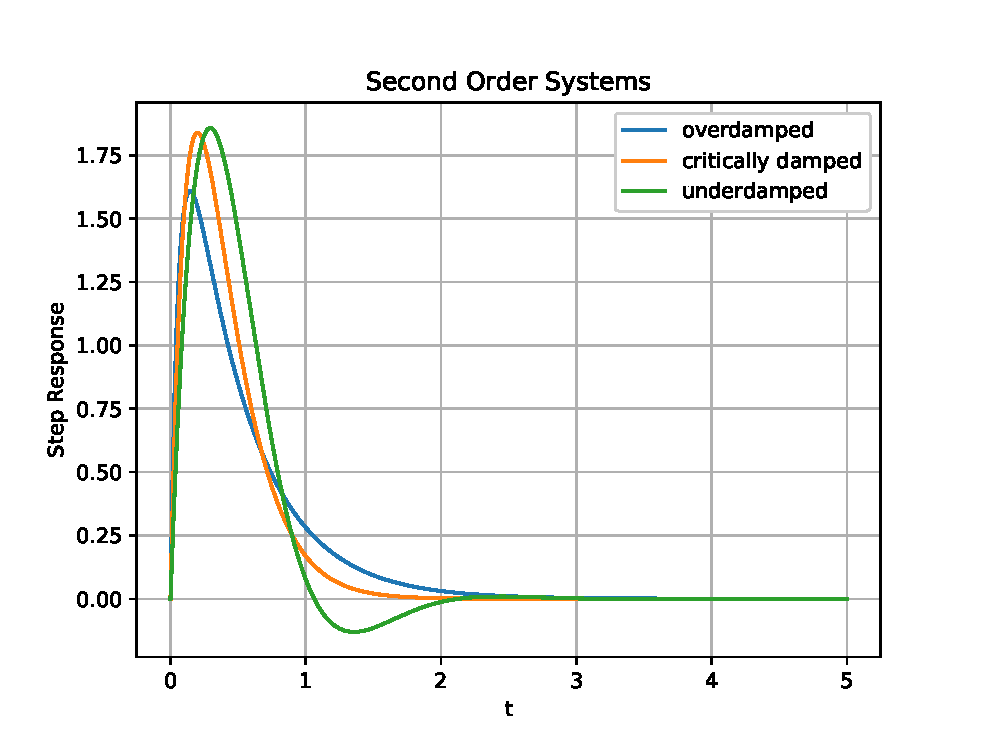
\includegraphics[width=\columnwidth]{./figs/ee18btech11012.eps}
    \caption{}
    \label{fig:ee18btech11012}
\end{figure}
%
The polar plot is to the right of $\brak{-1,0}$.  Hence the closed loop system is stable.
%
\end{enumerate}
